%\documentclass[aspectratio=169]{beamer}
% use this if you don't want the bookmark tab to show up on the left
% by default, it's true
\documentclass[hyperref={bookmarks=false}]{beamer}	
%\documentclass[aspectratio=43]{beamer}
\usepackage{tikz}
\usetikzlibrary{calc,trees,positioning,arrows,chains,shapes.geometric,%
decorations.pathreplacing,decorations.pathmorphing,shapes,%
matrix,shapes.symbols}

\mode<presentation> {
	\usetheme{Madrid}

  
	% \usetheme{CambridgeUS}
}

\usepackage[ampersand]{easylist}
\usepackage{bookmark,booktabs,comment,graphicx,subcaption,epsfig,amsfonts,amsmath,amssymb,mathrsfs,color,enumerate,empheq,wrapfig,empheq,epstopdf}
\numberwithin{figure}{section}

\DeclareMathOperator*{\tr}{tr}
\DeclareMathOperator*{\blockdiag}{blockdiag}
\DeclareMathOperator*{\sgn}{sgn}

\usefonttheme{serif}	% make letters/symbols that should be boldfaced boldface

\input{Symbol_Shortcut.tex}

\title{MMSE Based MIMO Channel Estimator Via Primal-Dual
Optimization Mehthod with Neural Network}
\author{Jing-Hao, Lee and Zhao-Jie, Luo}
\institute[NYCU] % Your institution as it will appear on the bottom of every slide, may be shorthand to save space
{
% \textit{janny00kevin@gmail.com} % Your email address
\\
\medskip
Advisor: Professor Carrson C. Fung\\ 
\medskip
National Yang Ming Chiao Tung University \\ % Your institution for the title page
}
\date{Jun. 12 2024}

\AtBeginSection[]
{
  \begin{frame}<beamer>
    \frametitle{Outline} %\insertsectionhead
    \tableofcontents[currentsection]
  \end{frame}
}
\setbeamertemplate{frametitle continuation}{(\insertcontinuationcount)}

\begin{document}
\frame{\titlepage}

%%%%%%%%%%%%%%%%%%%%%%%%%%%%%%%%%%%%%%%%%%%%%%%%%%%%%%%%%%%%%%%%%%
\begin{frame}{Reference}
%%%%%%%%%%%%%%%%%%%%%%%%%%%%%%%%%%%%%%%%%%%%%%%%%%%%%%%%%%%%%%%%%%
\begin{enumerate}
    \item C. C. Fung, and D. Ivakhnenkov, "Model-Driven Neural Network Based MIMO Channel Estimator".
    \item M. Eisen and A. Ribeiro, ``Large scale wireless power allocation with graph neural networks,'' \emph{Proc. of the 2019 IEEE 20th Workshop on Signal Processing Advances in Wireless Communications (SPAWC)}, pp. 1-5, 2019.
    \item M. Eisen, C. Zhang, L.F.O. Chamon, D.D. Lee and A. Ribeiro, ``Learning optimal power allocations in wireless systems,'' \emph{IEEE Trans. on Signal Processing}, vol. 67(10), pp. 2775-2790, May 2019.
    \item M. Eisen and A. Ribeiro, ``Optimal wireless resource allocation with random edge graph neural networks,'' \emph{IEEE Trans. on Signal Processing}, vol. 68, pp. 2977-2991, 2020.
    \item N. NaderiAlizadeh, M. Eisen and A. Ribeiro, ``State-Augmented learnable algorithms for resource management in wireless networks,'' \emph{IEEE Trans. on Signal Processing}, vol. 70, pp. 5898-5912, Dec. 2022.
    \item N. NaderiAlizadeh, M. Eisen and A. Ribeiro, ``Learning resilient radio resource management policies with graph neural networks,'' \emph{IEEE Trans. on Signal Processing}, volo. 71, pp. 995-1009, Mar. 2023.
    % \item S. Shi \emph{et al.}, ``MMSE optimization with per-base-station power constraints for network MIMO systems'', \emph{Proc. of the IEEE Intl. Conf. on Communications}, pp. 4106-4110, Bejing, China, May 2008
\end{enumerate}
% \bibstyle{abbrv}
%     \begin{thebibliography}{1}
%     \bibitem{Carrson}
%         C. C. Fung, and D. Ivakhnenkov, "Model-Driven Neural Network Based MIMO Channel Estimator".
%     \bibitem{Eisen2019conf}
%         M. Eisen and A. Ribeiro, ``Large scale wireless power allocation with graph neural networks,'' \emph{Proc. of the 2019 IEEE 20th Workshop on Signal Processing Advances in Wireless Communications (SPAWC)}, pp. 1-5, 2019.
%     \bibitem{Eisen2019journal}
%         M. Eisen, C. Zhang, L.F.O. Chamon, D.D. Lee and A. Ribeiro, ``Learning optimal power allocations in wireless systems,'' \emph{IEEE Trans. on Signal Processing}, vol. 67(10), pp. 2775-2790, May 2019.
%     \bibitem{Eisen2020}
%         M. Eisen and A. Ribeiro, ``Optimal wireless resource allocation with random edge graph neural networks,'' \emph{IEEE Trans. on Signal Processing}, vol. 68, pp. 2977-2991, 2020.
%     \bibitem{Naderi2022}    
%         N. NaderiAlizadeh, M. Eisen and A. Ribeiro, ``State-Augmented learnable algorithms for resource management in wireless networks,'' \emph{IEEE Trans. on Signal Processing}, vol. 70, pp. 5898-5912, Dec. 2022.
%     \bibitem{Naderi2023}    
%         N. NaderiAlizadeh, M. Eisen and A. Ribeiro, ``Learning resilient radio resource management policies with graph neural networks,'' \emph{IEEE Trans. on Signal Processing}, volo. 71, pp. 995-1009, Mar. 2023.
%     % \bibitem{Naderi2024}
%     %     S. Das, N. NaderiAlizadeh and A. Ribeiro, ``State-augmented information routing in communication systems with graph neural networks,''  \emph{IEEE Intl. Conf. on Acoustics, Speech and Signal Processing (ICASSP)}, Seoul, South Korea, Apr. 2024.
%         % OpenAI Spinning Up introduction to RL Part 3: Intro to Policy Optimization %: \href{https://spinningup.openai.com/en/latest/spinningup/rl_intro3.html}
%     \end{thebibliography}

\end{frame}


%%%%%%%%%%%%%%%%%%%%%%%%%%%%%%%%%%%%%%%%%%%%%%%%%%%%%%%%%%%%%%%%%%
\begin{frame}{Problem Setup}
%%%%%%%%%%%%%%%%%%%%%%%%%%%%%%%%%%%%%%%%%%%%%%%%%%%%%%%%%%%%%%%%%%

The system model can be represented as:
    \begin{equation} \label{eq:sysModel}
        \Y = \H\X + \W,
    \end{equation}
where $\X \in \mathbb{C}^{n_T \times T}$ represents the transmitted pilot signal, $\W \in \mathbb{C}^{n_R \times T}$ represents the additive white Gaussian noise
with zero mean and unit variance, $\Y \in \mathbb{C}^{n_R \times T}$ represents the received signal, and $\H \in \mathbb{C}^{n_R \times n_T}$ 
is the channel matrix containing channel coefficients which represents $n_R \times n_T$ flat fading channel.

Vectorizing (\ref{eq:sysModel}), it becomes 
    \begin{align} \label{vecSysModel}
        \y &= (\X \otimes \I_{n_R})\h + \w \notag \\ &= \tilde{\X}\h + \w,
    \end{align}
    where $\tilde{\X} \triangleq (\X \otimes \I_{n_R}) \in \mathbb{C}^{n_T n_R \times T n_R}.$

\end{frame}

%%%%%%%%%%%%%%%%%%%%%%%%%%%%%%%%%%%%%%%%%%%%%%%%%%%%%%%%%%%%%%%%%%
\begin{frame}{Problem Formulation}
%%%%%%%%%%%%%%%%%%%%%%%%%%%%%%%%%%%%%%%%%%%%%%%%%%%%%%%%%%%%%%%%%%

The MMSE channel estimator aims to minimize the Bayesian MSE of the channel estimate $\hat{\h}$ 
\begin{equation} \label{eq:mmse1}
    \hat{\h} = \argmin_{\hat{\h}} \mathrm{BMSE}(\hat{\h}),
\end{equation}
where
\begin{equation} \label{eq:bmse}
    \mathrm{BMSE}(\hat{\h}) = \mathbb{E}_{\y,\h}\left[\left\| \h-\hat{\h} \right\|^2_2\right].
\end{equation}
The closed-form solution of this MMSE problem is $\hat{\h} = \mathbb{E}_{\h|\y}\left[\h|\y\right]$. However, it requires knowledge about the conditional probability
$p(\h|\y)$, which may be unknown and/or difficult to obtain. Then (\ref{eq:mmse1}) can be written as
\begin{equation} \label{eq:mmse2}
    \min_{\hat{\h}} \mathbb{E}_{\y,\h}\left[\left\| \h-\hat{\h} \right\|^2_2\right].
\end{equation}\\

% Our objective is to minimize the expected mean square error:
% \begin{align*}
%     \min_{\hat{\h}} \mathbb{E}_{\y,\h}\left[\left\| \h-\hat{\h} \right\|^2_2 \right]\\
% \end{align*}
% and it can be written in epigraph form as:
% \begin{align*}
%     \min_{t,\h} {t}\\
%     s.t. &\ \mathbb{E}_{\y,\h}\left[\left\| \h-\hat{\h} \right\|^2_2 \right] \leq t\\
% \end{align*}

\end{frame}

%%%%%%%%%%%%%%%%%%%%%%%%%%%%%%%%%%%%%%%%%%%%%%%%%%%%%%%%%%%%%%%%%%
\begin{frame}[allowframebreaks]{Primal-Dual Optimization Mehthod}
%%%%%%%%%%%%%%%%%%%%%%%%%%%%%%%%%%%%%%%%%%%%%%%%%%%%%%%%%%%%%%%%%%

(\ref{eq:mmse2}) can be reformulated to its epigraph form as
\begin{equation}
\begin{aligned} \label{eq:epi}
    \min_{t,\hat{\mathbf{h}}} \quad & t \\
    \text{s.t.} \quad & \mathbb{E}_{\mathbf{y},\mathbf{h}}\left[\left\| \mathbf{h}-\hat{\mathbf{h}} \right\|^2_2\right] \leq t.
\end{aligned}
\end{equation}
Then its Lagrangian function can be written as
\begin{equation} \label{eq:Lag1}
    \mathcal{L} \left(\hat{\h},t,\lambda\right) = t + \lambda\left(\mathbb{E}_{\y,\h}\left[\left\| \h-\hat{\h} \right\|^2_2 \right] -t \right)
\end{equation}

\framebreak

We use parameterize channel estimator so that $\hat{\h}=\phi(\mathbf{y};\boldsymbol{\theta})$, 
with $\boldsymbol{\theta}$ denoting the parameters of the neural network.
\\ \hspace*{\fill} \\
Then the Lagrangian function of (15) can be written as
\begin{equation*}
    \begin{split}
        \mathcal{L} \left(\hat{\h},t,\lambda\right)
        &= t + \lambda\left(\mathbb{E}_{\y,\h}\left[\left\| \h-\hat{\h} \right\|^2_2 \right] -t \right)\\
        &= t + \lambda\left(\mathbb{E}_{\y,\h}\left[\left\| \h-\phi(\mathbf{y};\boldsymbol{\theta}) \right\|^2_2 \right] -t \right)
    \end{split}
\end{equation*}
\framebreak

It is uncertain whether or not the duality gap equals zero.\\
However, the stationary point of $  \mathcal{L} \left(\hat{\h},t,\lambda\right)$
can be found via the KKT conditions by solving for the primal and dual
variables alternately using gradient descent and ascent, respectively:

\begin{equation*}
    \begin{split}
        \boldsymbol{\theta}_{k+1} &= \boldsymbol{\theta}_{k} - 
            \alpha_{\boldsymbol{\theta},k} \lambda_k \nabla_{\boldsymbol{\theta}_k}
            \mathbb{E}\left[\left\| \h-\phi(\mathbf{y};\boldsymbol{\theta}_k) \right\|^2_2 \right]\\
        t_{k+1} &= t_{k} - \alpha_{t,k}(1-\lambda_k)\\
        \lambda_{k+1} &= \left[ \lambda_k + \alpha_{\lambda,k}
            \left( \mathbb{E}\left[\left\| \h-\phi(\mathbf{y};\boldsymbol{\theta}_{k+1}) \right\|^2_2 \right] 
            -t_{k+1}\right)\right]_{+}
    \end{split}
\end{equation*}

\end{frame}


%%%%%%%%%%%%%%%%%%%%%%%%%%%%%%%%%%%%%%%%%%%%%%%%%%%%%%%%%%%%%%%%%%
\begin{frame}[allowframebreaks]{Policy Gradient}
%%%%%%%%%%%%%%%%%%%%%%%%%%%%%%%%%%%%%%%%%%%%%%%%%%%%%%%%%%%%%%%%%%

The policy gradient theorem is:
\begin{align*}
    \nabla_{\boldsymbol{\theta}}\mathbb{E}_{\tau}[G(\tau)]
        =\mathbb{E}_{\tau}\left[\sum\limits_{t=0}^{T-1}G(\tau)
        \nabla_{\boldsymbol{\theta}}\log{\pi_{\boldsymbol{\theta}}
        (A_t|S_t)}\right],
\end{align*}
where $G(\tau)$ is the overall return of the trajectory, and $\pi_{\boldsymbol{\theta}(A_t|S_t)}$ is the distribution of action that 
        the parameterized policy makes under the observation. 

At each time step, $t=1,...,T-1$:
\begin{align*}
    \nabla_{\boldsymbol{\theta}}\mathbb{E}_{\tau}[G(\tau)]
        =\mathbb{E}_{\tau}\left[G(\tau)
        \nabla_{\boldsymbol{\theta}}\log{\pi_{\boldsymbol{\theta}}
        (A_t|S_t)}\right]
\end{align*}

And we can estimate the policy gradient with sample mean:
\begin{align*}
    \widehat{\nabla_{\boldsymbol{\theta}}}\mathbb{E}_{\tau}[G(\tau)]
        =\frac{1}{\left| \mathcal{D}  \right|} \sum\limits_{\mathcal{D}}
        G(\tau)\nabla_{\boldsymbol{\theta}}\log{\pi_{\boldsymbol{\theta}}
        (A_t|S_t)}
\end{align*}

%%%%%%%%%%%%%%%%%%%%%%%%%%%%%%%%%%%%%%%%%%%%%%%%%%%%%%%%%%%%%%%%%%
\framebreak

Our goal is to minimize the mean square error, by substituting 
$\mathbb{E}_{\tau}[G(\tau)]$, $\pi_{\boldsymbol{\theta}}(A_t|S_t)$ with 
$\mathbb{E}_{\y,\h}\left[\left\| \h-\phi(\mathbf{y};\boldsymbol{\theta}) \right\|^2_2 \right]$,
and $\pi_{\boldsymbol{\theta}}(\hat{\h}|\y)$.\\
Thus, we obtain the estimated policy gradient for our problem:
\begin{equation} \label{policy gradient}
    \widehat{\nabla_{\boldsymbol{\theta}}}
            \mathbb{E}_{\y,\h}\left[\left\| \h-\phi(\mathbf{y};\boldsymbol{\theta}) \right\|^2_2 \right]
            = \frac{1}{\left| \mathcal{D}  \right|} \sum\limits_{\mathcal{D}}
            \left\| \h-\widehat{\phi}(\mathbf{y};\boldsymbol{\theta}) \right\|^2_2
            \nabla_{\boldsymbol{\theta}}
            \log \pi_{\boldsymbol{\theta}}
            \left( \hat{\h}|\y \right)
\end{equation}
where $\hat{\phi}(\mathbf{y};\boldsymbol{\theta}) = 
\hat{\h}$ is the sampled output of the policy. 

\end{frame}


%%%%%%%%%%%%%%%%%%%%%%%%%%%%%%%%%%%%%%%%%%%%%%%%%%%%%%%%%%%%%%%%%%
\begin{frame}{Experiment Diagram}
%%%%%%%%%%%%%%%%%%%%%%%%%%%%%%%%%%%%%%%%%%%%%%%%%%%%%%%%%%%%%%%%%%
\begin{figure}
  \centering
  \begin{tikzpicture}[start chain=going below, node distance=50pt]
      \node[] (a) {};
      \node[draw, right=3.5cm of a] (MLP) {MLP};
      \node[draw, right=2cm of MLP] (sample) {sample};
      \draw [->] (MLP) -- node[name=N, align=center,font=\scriptsize] 
              {$\mathcal{N}(\mu_i,\sigma_i)$\\
              \fontsize{6}{6}\selectfont$i=1,...,
              2n_Rn_T$} (sample);
      \node[draw, above=4cm of N] (batch) {batch};
      \node[draw, below of=N, align=center,font=\small]   (env) 
              {Environment \\ \fontsize{9}{12}\selectfont $\Y=\H\X+\W$};
      \draw [->] (sample) --(10,0)--(10,4.7)-- (batch);
      \draw [->] (env) --(1.8,-1.75)--(1.8,4.7)-- (batch);
      \draw [->] (env) --(5.75,-2.5)--(1,-2.5)--(1,5.25)--(5.75,5.25)-- (batch);
      \draw [-]  (1,-2.5)--node[name=H,align=center] {$\h\quad$} (1,5.25);
      \draw [->] (1.8,0) --node[name=Y,align=center,font=\footnotesize]
              {$\y \in \mathbb{R}^{2n_RT}$\\} (MLP);
      \draw [->] (batch) --(5.75,4)--(2.75,4)--(2.75,1)--(4.2,1)-- (MLP);
      \draw [-,] (sample) --node[name=Hhat,align=center,font=\footnotesize] 
              {$\hat{\h}\in\mathbb{R} ^{2n_Tn_R}$\\} (10,0);
      \node [font=\tiny] at (6.15,3) {$\lambda_{k+1} = \left[ \lambda_k + \alpha_{\lambda,k}
              \left( \frac{1}{\left| \mathcal{D}  \right|} \sum\limits_{\mathcal{D}} \left\| \h-\widehat{\phi}(\mathbf{y};\boldsymbol{\theta}_{k}) \right\|^2_2
              -t_{k}\right)\right]_{+}$};
      \node [font=\tiny] at (5.65,2.5) {$\boldsymbol{\theta}_{k+1} = \boldsymbol{\theta}_{k} - 
              \alpha_{\boldsymbol{\theta},k} \lambda_k \widehat{\nabla}_{\boldsymbol{\theta}_k}
              \mathbb{E}\left[\left\| \h-\phi(\mathbf{y};\boldsymbol{\theta}_k) \right\|^2_2 \right]$};
      \node [font=\tiny] at (4.6,2) {$t_{k+1} = t_{k} - \alpha_{t,k}(1-\lambda_{k+1})$};
      \node [align=left] at (8.3,-1.75) 
              {\parbox[b]{1.7cm}{\fontsize{6}{6}\selectfont 
                  $\Y \in \mathbb{C}^{n_R \times T}$\\
                  $\H \in \mathbb{C}^{n_R \times n_T}$\\
                  $\X \in \mathbb{C}^{n_T \times T}$\\
                  $\W \in \mathbb{C}^{n_R \times T}$}
              };
      % \node at (0,0) {\parbox[b]{3cm}{\fontsize{24}{28}\selectfont Large Text\\ \fontsize{12}{14}\selectfont Normal Text}};
  \end{tikzpicture}
  % \caption{exp diagram}
  \label{fig:exp diagram}
\end{figure}

\end{frame}

%%%%%%%%%%%%%%%%%%page2%%%%%%%%%%%%%%%%%%%%%%
\begin{frame}{GNN}
\begin{itemize}
    \item \footnote{M. Eisen and A. Ribeiro, “Optimal wireless resource allocation with random edge graph neural networks,” IEEE Trans. on
    Signal Processing, vol. 68, pp. 2977-2991, 2020.}How to optimally allocating resources across a set of transmitters and receivers in a a wireless network?
    \item This paper proposes a method using REGNN.
    \item The performance of using REGNN is better than using MLP
        \begin{enumerate}
            \item number of parameter
            \item time complexity
            \item scalability
            \item transference
        \end{enumerate}
    \item Therefore, we introduce the GNN method to replace MLP for estimating channel H.
\end{itemize}
    
\end{frame}

%%%%%%%%%%%%%%%%%%page3%%%%%%%%%%%%%%%%%%%%%%
\begin{frame}{GNN}
\begin{itemize}
    \item $F_{\ell}$ : the number of the filters at $\ell$ layer. 
    \item L : total layer of GNN.
    \item $K_{\ell}$ : the order of the filters at $\ell$ layer.
    % \begin{equation}
    % \item 
    \begin{align}
        F_{\ell}^{I/O}(\W) 
        &= \displaystyle\sum^{K_{\ell}-1}_{k=0}a_{\ell/k}^{I/O}\W^{k} \\
        &= a_{\ell/0}^{I/O}\I + a_{\ell/1}^{I/O}\W + a_{\ell/2}^{I/O}\W^{2} + \ldots + a_{\ell/K_{\ell-1}}^{I/O}\W^{K_{\ell}-1} \\
        & \text{where }  \ell:\text{layer, } I:\text{input index, } O:\text{output index }
    \end{align}
    \item Example : 
    \begin{align}
        F_{0}^{1/3}(\W) &= \displaystyle\sum^{2}_{k=0}a_{0/k}^{1/3}\W^{k} \\
        &= a_{0/0}^{1/3}\I + a_{0/1}^{1/3}\W + a_{0/2}^{1/3}\W^{2}
    \end{align}
    % \end{equation}
    % \item $F_{\ell}^{I/O}(\W)$ = $\displaystyle\sum^{K_{\ell}-1}_{k=0}a_{\ell/k}^{I/O}\W^{k} \\
    % \hspace{1mm}= a_{\ell/0}^{I/O}\I + a_{\ell/1}^{I/O}\W + a_{\ell/2}^{I/O}\W^{2} + \ldots + a_{\ell/K_{\ell-1}}^{I/O}\W^{K_{\ell}-1} \\
    % \hspace{1mm} where $\ell$:layer, I:input index, O:output index$
\end{itemize}
% \begin{itemize}
% \end{itemize}
\end{frame}
%%%%%%%%%%%%%%%%%%page4%%%%%%%%%%%%%%%%%%%%%%
\begin{frame}{GNN}
\begin{itemize}
    \item $K_{\ell} = 3, L = 2, F_{1} = 3, F_{2} = 8$, $n_{T}$ = 2, $n_{R}$ = 2
\end{itemize}
\includegraphics[width=4.3in,height=2.5in]{figures/REGNN_V2.jpg}
\begin{itemize}
    \item Total parameter : 3x3+3x3x8 = 81
\end{itemize}
\end{frame}
%%%%%%%%%%%%%%%%%%page5%%%%%%%%%%%%%%%%%%%%%%
\begin{frame}{BUT!}
\begin{itemize}
    \item It is not possible to use the adjacency matrix (Channel matrix, \H) as the Graph Shift Operator because the Channel matrix is the output of the REGNN, and we do not know $\H$ initially.
    \item Because in Eisen's paper, the Channel matrix $\H$ is known, the adjacency matrix is also known, which means the Graph Shift Operator can be used for convolution.
    \item Therefore, it might be impossible to use GNN methods to solve our problem.
\end{itemize}
\end{frame}
%%%%%%%%%%%%%%%%%%page6%%%%%%%%%%%%%%%%%%%%%%
\begin{frame}{Guess}
\begin{itemize}
    \item Since we don't have $\H$, we use Least-Square estimator to find $\H_{initial}$. With this $\H_{initial}$,we can determine the adjacency matrix, which gives us the GSO. Then, we can use the GNN output to obtain $\hat{\H}$. If the performance of this $\hat{\H}$ is not satisfactory, we can use $\hat{\H}$ to determine a new adjacency matrix as the GSO and use the GNN again to obtain another $\hat{\H}$. We can repeat this process until the performance approaches that of the MMSE estimator.
\end{itemize}
\end{frame}
%%%%%%%%%%%%%%%%%%page7%%%%%%%%%%%%%%%%%%%%%%
\begin{frame}{Guess}
\begin{itemize}
    \item As illustrated in the diagram below.
\end{itemize}
\centering
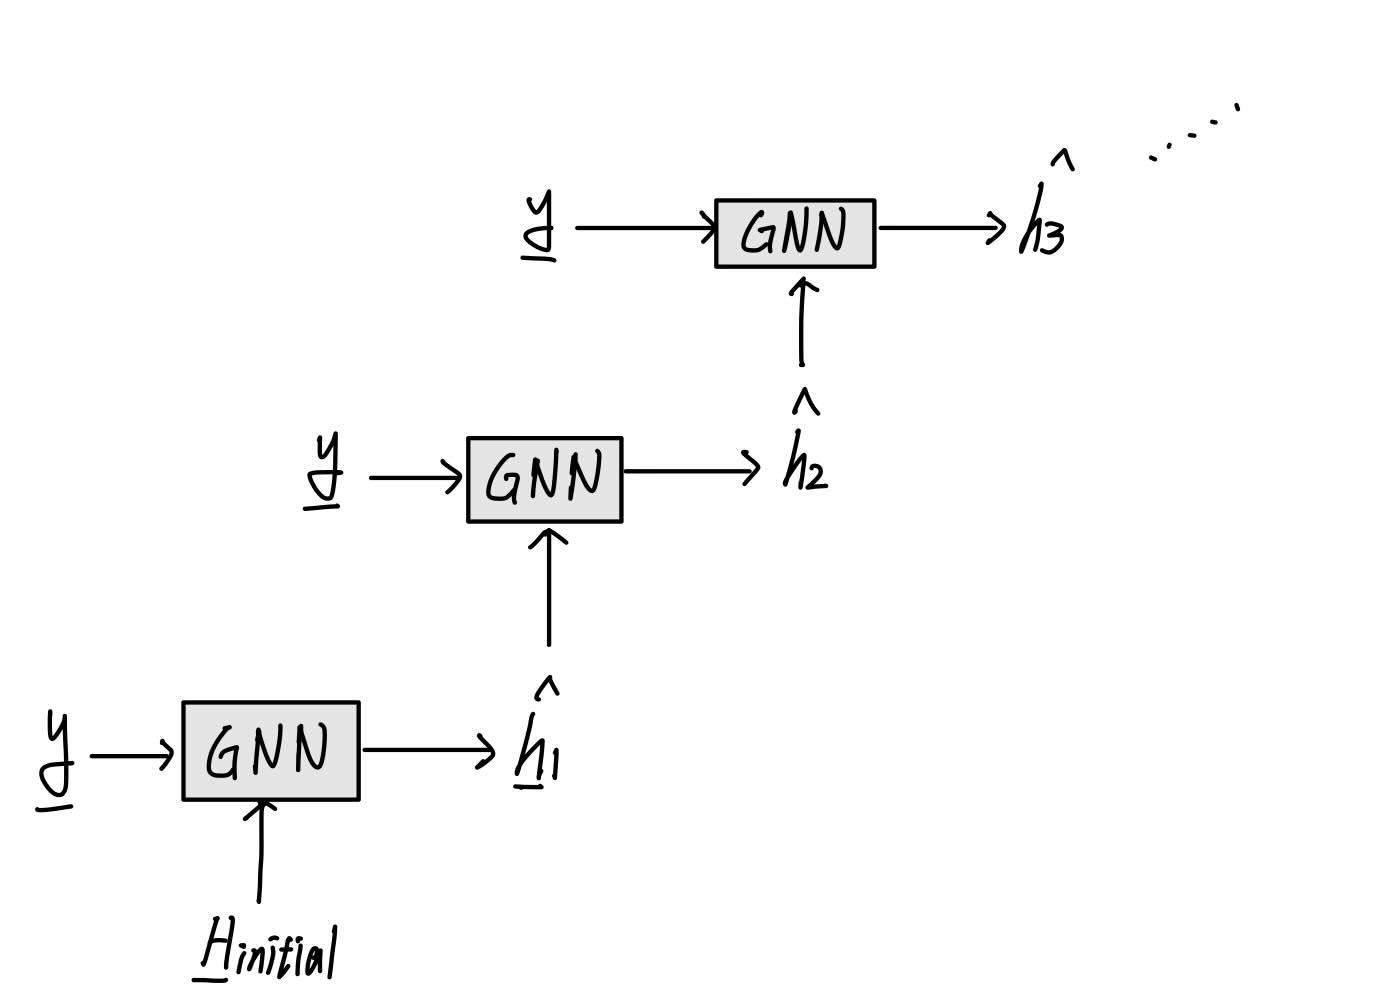
\includegraphics[width=3.5in,height=2.0in]{figures/Guess.jpg}
\begin{itemize}
    \item I guess that using this method, the estimated $\hat{\H}$ will get increasingly better.
\end{itemize}
\end{frame}


%%%%%%%%%%%%%%%%%%%%%%%%%%%%%%%%%%%%%%%%%%%%%%%%%%%%%%%%%%%%%%%%%%
\begin{frame}[allowframebreaks]{Simulation Configuration}
%%%%%%%%%%%%%%%%%%%%%%%%%%%%%%%%%%%%%%%%%%%%%%%%%%%%%%%%%%%%%%%%%%

\begin{table}[H] \label{tab:Configuration}
    \centering
    \renewcommand{\arraystretch}{1.2}
    \begin{tabular}{|c|c|}
        \hline
        parameters   &values \\
        \hline \hline
        [$n_R,n_T$,$T$]                 &[4,8,8]        \\ \hline
        $\mu_H, \sigma_H$               &0, 1          \\ \hline
        Hidden layer size               &1024 or 4$\times$1024   \\ \hline
        Length of each trajectory       &1                      \\ \hline
        Batch size = $|\mathcal{D}|$    &10,000         \\ \hline
        Number of batches               &100            \\ \hline
        Trainning dataset               &1,000,000      \\ \hline
        Validation dataset              &2,000          \\ \hline
        Epoch                           &200 $\sim$ 1,000   \\ \hline
        Learning rate                   &1e-5 $\sim$ 1e-6  \\ \hline
    \end{tabular}
    \caption{simulation configuration}
\end{table}

\framebreak
%%%%%%%%%%%%%%%%%%%%%%%%%%%%%%%%%%%%%%%%%%%%%%%%%%%%%%%%%%%%%%%%%%

\begin{itemize}
    \item Let the loss be Normalized Mean Squared Error (NMSE):
        \begin{equation} \label{NMSE}
          NMSE=\frac{1}{N} \sum\limits_{n=1}^N
          \frac{\left\| \h_n-\phi(\mathbf{y}_n;\boldsymbol{\theta}_k) \right\|^2_2}
          {\left\| \h_n \right\|^2_2}
        \end{equation}
        Here, $N$ represents the size of the training or validation dataset, 
        implying that the Normalized Mean Squared Error (NMSE) is calculated for each epoch.
    \vspace{12pt}
    \item Using Adam optimizer to update the primal and dual variables.
 
\end{itemize}
\end{frame}

%%%%%%%%%%%%%%%%%%%%%%%%%%%%%%%%%%%%%%%%%%%%%%%%%%%%%%%%%%%%%%%%%%
\begin{frame}[allowframebreaks]{Simulation Result}
%%%%%%%%%%%%%%%%%%%%%%%%%%%%%%%%%%%%%%%%%%%%%%%%%%%%%%%%%%%%%%%%%%

\begin{figure}[H]
    \centering
    \begin{subfigure}[b]{.8\linewidth}
        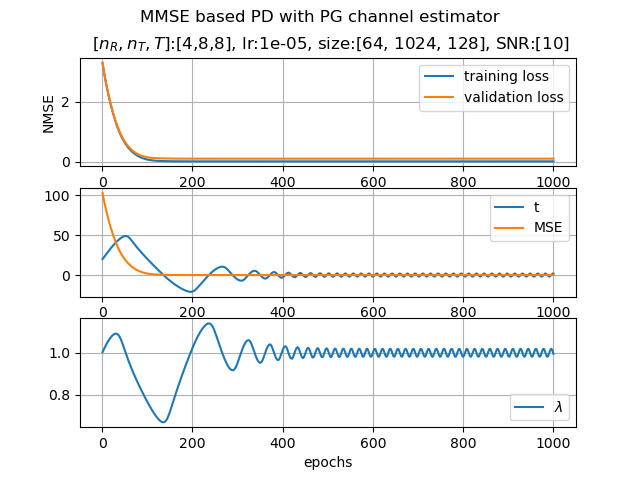
\includegraphics[width=\linewidth]{figures/lr1e-05_[64, 1024, 128]_ep1000_SNR_[10].png}
    %   \caption{lr: 1e-3, epoch: 100}
    %   \label{fig:image1}
    \end{subfigure}
    \begin{subfigure}[b]{.8\linewidth}
        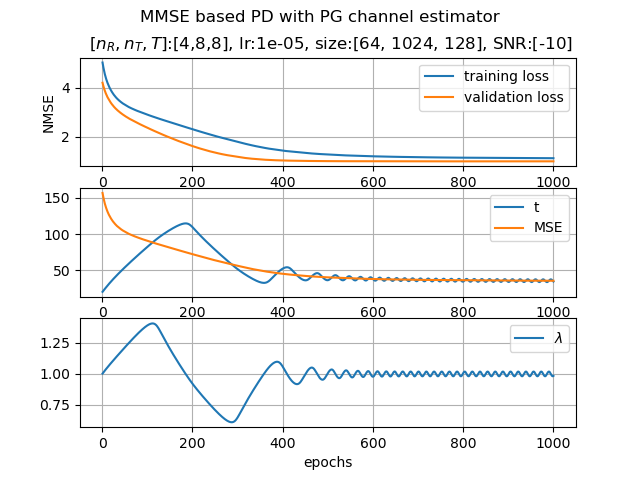
\includegraphics[width=\linewidth]{figures/lr1e-05_[64, 1024, 128]_ep1000_SNR_[-10].png}
    %   \caption{lr: 1e-3, epoch: 100}
    %   \label{fig:image2}
    \end{subfigure}
    \begin{subfigure}[b]{.8\linewidth}
        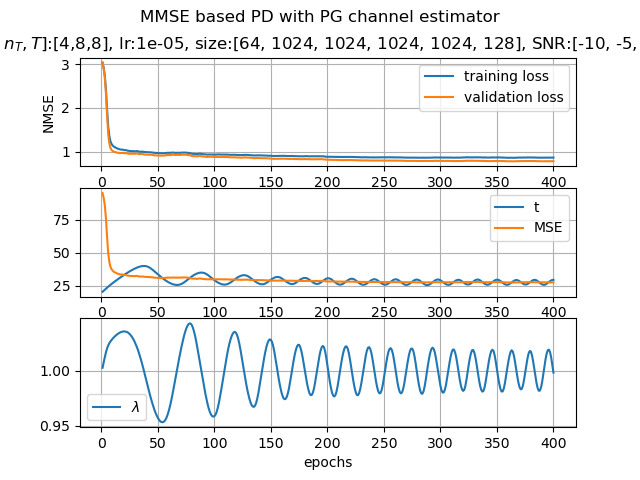
\includegraphics[width=\linewidth]{figures/lr1e-05_[64, 1024, 1024, 1024, 1024, 128]_ep400_SNR_[-10, -5, 5, 10].png}
    %   \caption{Image 3}
    %   \label{fig:image3}
    \end{subfigure}
    % \caption{(a) 1 hidden layer MLP trained with SNR = 10
    %     (b) 1 hidden layer MLP trained with SNR = -10
    %     (c) 4 hidden layer MLP trained with SNR = -10, -5, 5, 10}
    \label{fig:train_result}
\end{figure}

\begin{figure}[h]
    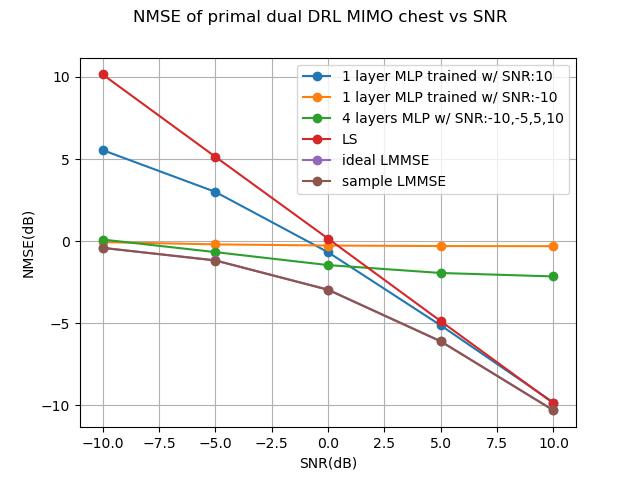
\includegraphics[width=.8\linewidth]{figures/3mlp_Chest_.png}
    % \caption{performance of channel estimators under different SNRs}
    \label{fig:test_result}
\end{figure}

% Figure (\ref{fig:test_result}) shows the testing results of MLPs from Figure (\ref{fig:train_result}) under different SNRs, 
%         compared with LS, sampled LMMSE, and ideal LMMSE estimators, where the ideal LMMSE is calculated using the ideal covariance matrix of $\H$: 
%         $\C_{\h\h}(\C_{\h\h}+\C_{\w\w})^{-1}\y = \sigma_{\H}^2\I(\sigma_{\H}^2\I + \sigma_{\W}^2\I)^{-1}\y = \frac{\sigma_{\H}^2}{\sigma_{\H}^2+\sigma_{\W}^2}\y$
%         and the sample LMMSE is calculated using $\H$ from testing dataset: $\C_{\h\h} = \frac{1}{N}\sum_{n=1}^{N}\h_n\h_n^T$, where $N$ is the size of testing dataset.

\end{frame}



%%%%%%%%%%%%%%%%%%%%%%%%%%%%%%%%%%%%%%%%%%%%%%%%%%%%%%%%%%%%%%%%%%
\begin{frame}{Conclusion}
%%%%%%%%%%%%%%%%%%%%%%%%%%%%%%%%%%%%%%%%%%%%%%%%%%%%%%%%%%%%%%%%%%

\begin{itemize}
\item Our simulation results demonstrate that the proposed neural network-based MMSE estimator can outperform the least squares (LS) and approach the performance of 
linear MMSE (LMMSE) estimators under specific signal-to-noise ratio (SNR) conditions, especially under challenging conditions with high noise levels. 

\item However, it may requires a larger model size or more sophisticated neural network architectures to achieve robustness in its performance.
\end{itemize}
\end{frame}

\end{document}
